\documentclass{article}
\newtheorem{thm}{Theorem}
\setlength{\oddsidemargin}{0.25in}
\setlength{\textwidth}{6in}
\setlength{\topmargin}{-0.25in}
\setlength{\headheight}{0.3in}
\setlength{\headsep}{0.2in}
\setlength{\textheight}{9in}
\setlength{\footskip}{0.1in}
\usepackage{multirow}
\usepackage{fullpage}
\usepackage{graphicx}
\usepackage{amsthm}
\usepackage{amssymb}
\usepackage{url}
\usepackage{amsfonts}
\usepackage{algpseudocode}
\usepackage{mathtools}
\usepackage{listings}
\newcommand{\quotes}[1]{``#1''}
\newcommand{\argmin}{\arg\!\min}
\newcommand{\argmax}{\arg\!\max}

\usepackage{hyperref}
\hypersetup{
    colorlinks=true,
    linkcolor=blue,
    filecolor=magenta,      
    urlcolor=blue,
}

\begin{document}\title{Homework 5\\ Introduction to Data Analysis and Mining \\ Spring 2018\\ CSCI-B 365}         % Enter your title between curly braces
\author{Instructor: Hasan Kurban}        % Enter your name between curly braces
\date{\today}          % Enter your date or \today between curly braces
\maketitle
\makeatother     % `@' is restored as a "non-letter" character
\pagestyle{plain}
\section*{Directions}
Please follow the syllabus guidelines in turning in your homework.  I am providing the \LaTeX{} of this document too. This homework is due Sunday, April 8, 2018 10:00p.m. \textbf{OBSERVE THE  TIME}. Absolutely no homework will be accepted after that time. All the work should be your own.  



 
   %%%%%%%%%%%%%%%%%%%%%%%%%%%%%%%%%%%%%%
%                      PROBLEM 1
 %%%%%%%%%%%%%%%%%%%%%%%%%%%%%%%%%%%%%%
 
 
\section*{K-Nearest Neighbors (KNN) Algorithm in Theory}
{\small
\begin{center}
\begin{algorithmic}[1]\label{alg:knn}
\State{\bf ALGORITHM} \texttt{K-nearest neighbors}
\State {\bf INPUT}\begin{itemize}
\item \textsf{training data} $\Delta$
\item \textsf{test data} $\Delta'$  
\item \textsf{distance metric} $d$, i.e., $d:\Delta^2\rightarrow \mathbb{R}_{\geq 0}$ 
\item \textsf{integer} $k$: \textsf{nearest neighbors number}
\end{itemize}
\State {\bf OUTPUT} 
\begin{itemize}
\item \textsf{class label of each} $z \in \Delta' $
\end{itemize}
\For {$z = (\mathbf{x}',y') \in \Delta'$}
\State  \textsf{Compute} $d(\mathbf{x},\mathbf{x}')$, \textsf{the distance between z and every example} $(\mathbf{x},y) \in \Delta$
\State  \textsf{Select} $\Delta_z \subseteq \Delta$, \textsf{the set of closest} $k$ \textsf{training examples to z}
\State \textsf{Voting:}
\begin{itemize}
\item \textsf{majority voting}:
$y' = \argmax_v  \sum_{(\mathbf{x_i},y_i)\in\Delta_z} I(v=y_i)$
\item \textsf{distance-weighted voting}: $y' = \argmax_v  \sum_{(\mathbf{x_i},y_i)\in\Delta_z} w_i \times I(v=y_i)$ \textsf{where} $ w_i = \frac{1}{d(\mathbf{x',x_i})^2}$
\end{itemize}
\EndFor
\end{algorithmic}
\end{center}}

\pagebreak

\section*{K-Fold Cross Validation for Model Selection }

{\small
\begin{center}
\begin{algorithmic}[1]\label{alg:crossValidation}
\State{\bf ALGORITHM} \texttt{k-fold cross validatiaon}
\State {\bf INPUT} \begin{itemize}
\item \textsf{training data} $\Delta = (\mathbf{x_1},y_1),\ldots,(\mathbf{x_m},y_m)$
\item  set of parameter values $\Theta$
\item  learning algorithm $\mathcal{H}$
\item  integer $k$
\end{itemize}
\State {\bf OUTPUT}\begin{itemize}
\item $\theta^* =\argmin_\theta [error(\theta)]$
\item $h_{\theta^*} = \mathcal{H}(\Delta;\theta^*)$ 
\end{itemize}
\State Randomly partition $\Delta$ into $\Delta_1,\ldots,\Delta_k$
\State  \texttt{***} $\Delta_1\cup\Delta_2\ldots \cup\Delta_k = \Delta$ and $\Delta_i \cap \Delta_j = \varnothing$ for $i \neq j \in [1,2,\ldots,k]$
\For{$\theta \in \Theta$}
\For {$i = 1\ldots k$}
\State  \texttt{***}  \textsf{Train a model for each training set}
\State $h_{i,\theta} = \mathcal{H}(\Delta \setminus \Delta_i;\theta)$
\EndFor
\State  \texttt{***}  \textsf{Use the trained models over $\Delta_i$ (test data sets) to evaluate the models for each parameter}
\State error$(\theta)= \frac{1}{k} \sum_{i=1}^{k} \mathcal{L}_{\Delta_i} (h_{i,\theta})$
\EndFor
\end{algorithmic}
\end{center}}
%%%%%%%%%%%%%%%%%%%%%%%%%%%%%%%%%%%%%%
In this homework, you are asked to train several classifiers  using $k$-nearest neighbors (KNN) and  naive bayes  algorithms over  car evaluation and credit approval data sets.  The links for the data sets are provided below:
  
 \begin{itemize}
\item \href{https://archive.ics.uci.edu/ml/datasets/car+evaluation}{Car Evaluation Data Set}
\item \href{https://archive.ics.uci.edu/ml/datasets/Credit+Approval}{Credit Approval Data Set }
\end{itemize}

%%%%%%%%%%%%%%%%%%%%%%%%%%%%%%%%%%%%%%
\section*{Problem 1: $K$-Fold Cross Validation [20 points]}

Create $5$ training and $5$ test data sets from each data set using  $5$-fold cross validation and save these $20$ files. You will use these data sets to answer the rest of the questions. You are allowed to use R packages for $k$- fold cross validation. However,\textit{ students who implement it will receive $15$ extra points from this question}.

%%%%%%%%%%%%%%%%%%%%%%%%%%%%%%%%%%%%%%
\section*{Problem 2: $K$-Nearest Neighbors (KNN)[40 points]} 

\textbf{2.1}  Implement KNN algorithm with two different distance functions. You can either use existing distance functions, i.e., Euclidean  or design your own.
\\
\\
\textbf{2.2}  Use the data sets created in problem 1 to determine the optimal $k$  over each data set for KNN algorithm. First, pick 5  different $k$ values and then calculate average error rate of  KNN classifiers over test data tests  for each $k$ to find the optimal $k$ for each data set and distance function. Report the average error rate for each $k$, distance function and data set.  What are the optimal $k$ and distance function for each data set?
\\
\\
\begin{lstlisting}
> myknn(car1te,car1tr,"car",euDist)
k =  2[1] 0.07826087 "tie"
k =  20[1] 0.115942
k =  50[1] 0.1507246
k =  100[1] 0.1710145
k =  150[1] 0.2086957
> myknn(car1te,car1tr,"car",mDist)
k =  2[1] 0.07826087 
k =  20[1] 0.1217391
k =  50[1] 0.1507246
k =  100[1] 0.2144928
k =  150[1] 0.2405797
> myknn(car2te,car2tr,"car",euDist)
k =  2[1] 0.09855072 
k =  20[1] 0.1014493
k =  50[1] 0.1333333
k =  100[1] 0.173913
k =  150[1] 0.1942029
> myknn(car2te,car2tr,"car",mDist)
k =  2[1] 0.09855072
k =  20[1] 0.1188406
k =  50[1] 0.1710145
k =  100[1] 0.1913043
k =  150[1] 0.2376812
> myknn(car3te,car3tr,"car",euDist)
k =  2[1] 0.1304348
k =  20[1] 0.1130435
k =  50[1] 0.1478261
k =  100[1] 0.1710145
k =  150[1] 0.173913
> myknn(car3te,car3tr,"car",mDist)
k =  2[1] 0.1304348
k =  20[1] 0.1304348
k =  50[1] 0.1652174
k =  100[1] 0.1971014
k =  150[1] 0.2144928
> myknn(car4te,car4tr,"car",euDist)
k =  2[1] 0.09275362 
k =  20[1] 0.1188406
k =  50[1] 0.1478261
k =  100[1] 0.1536232
k =  150[1] 0.173913
> myknn(car4te,car4tr,"car",mDist)
k =  2[1] 0.09275362
k =  20[1] 0.1304348
k =  50[1] 0.1507246
k =  100[1] 0.1768116
k =  150[1] 0.2
> myknn(car5te,car5tr,"car",euDist)
k =  2[1] 0.07826087 "tie"
k =  20[1] 0.08985507
k =  50[1] 0.115942
k =  100[1] 0.1391304
k =  150[1] 0.1710145
> myknn(car5te,car5tr,"car",mDist)
k =  2[1] 0.07826087 "tie"
k =  20[1] 0.08985507
k =  50[1] 0.1217391
k =  100[1] 0.1507246
k =  150[1] 0.2057971
> myknn(cre1te,cre1tr,"credit",euDist)
k =  2[1] 0.4202899
k =  20[1] 0.3768116
k =  50[1] 0.2971014
k =  100[1] 0.3333333
k =  150[1] 0.3405797
> myknn(cre1te,cre1tr,"credit",mDist)
k =  2[1] 0.3188406
k =  20[1] 0.3043478
k =  50[1] 0.2971014
k =  100[1] 0.326087
k =  150[1] 0.3188406
> myknn(cre2te,cre2tr,"credit",euDist)
k =  2[1] 0.3115942
k =  20[1] 0.3043478
k =  50[1] 0.326087
k =  100[1] 0.3043478
k =  150[1] 0.326087
> myknn(cre2te,cre2tr,"credit",mDist)
k =  2[1] 0.2826087
k =  20[1] 0.2536232
k =  50[1] 0.2971014
k =  100[1] 0.3043478
k =  150[1] 0.3188406
> myknn(cre3te,cre3tr,"credit",euDist)
k =  2[1] 0.3623188
k =  20[1] 0.3333333
k =  50[1] 0.3550725
k =  100[1] 0.3695652
k =  150[1] 0.3985507
> myknn(cre3te,cre3tr,"credit",mDist)
k =  2[1] 0.2971014
k =  20[1] 0.2971014 
k =  50[1] 0.3478261
k =  100[1] 0.3768116
k =  150[1] 0.3768116
> myknn(cre4te,cre4tr,"credit",euDist)
k =  2[1] 0.326087
k =  20[1] 0.2391304 "tie"
k =  50[1] 0.2608696
k =  100[1] 0.2826087
k =  150[1] 0.2898551
> myknn(cre4te,cre4tr,"credit",mDist)
k =  2[1] 0.2971014
k =  20[1] 0.2536232
k =  50[1] 0.2391304 "tie"
k =  100[1] 0.2608696
k =  150[1] 0.2753623
> myknn(cre5te,cre5tr,"credit",euDist)
k =  2[1] 0.4057971
k =  20[1] 0.3333333
k =  50[1] 0.3115942
k =  100[1] 0.326087
k =  150[1] 0.326087
> myknn(cre5te,cre5tr,"credit",mDist)
k =  2[1] 0.2898551
k =  20[1] 0.2898551 
k =  50[1] 0.3115942
k =  100[1] 0.3043478
k =  150[1] 0.3188406

\end{lstlisting}
\textbf{2.3} Use the KNN package in R  to validate your results from question 2.2.
\begin{lstlisting}
car data1
k = 2 error= 0.05217391
k = 20 error= 0.1014493 
k = 50 error= 0.1391304 
k = 100 error= 0.1797101 
k = 150 error= 0.2231884 
car data2
k = 2 error= 0.04347826 
k = 20 error= 0.08985507 
k = 50 error= 0.1333333 
k = 100 error= 0.1768116 
k = 150 error= 0.2173913 
car data3
k = 2 error= 0.06376812 
k = 20 error= 0.1101449 
k = 50 error= 0.1507246 
k = 100 error= 0.173913 
k = 150 error= 0.1855072 
car data4
k = 2 error= 0.04927536 
k = 20 error= 0.09275362 
k = 50 error= 0.1449275 
k = 100 error= 0.1478261 
k = 150 error= 0.1768116 
car data5
k = 2 error= 0.02608696 "best"
k = 20 error= 0.07826087 
k = 50 error= 0.1130435 
k = 100 error= 0.1449275 
k = 150 error= 0.1797101 
credit data1
k = 2 error= 0.3478261 
k = 20 error= 0.3550725 
k = 50 error= 0.3043478
k = 100 error= 0.3405797 
k = 150 error= 0.3405797 
credit data2
k = 2 error= 0.3623188 
k = 20 error= 0.3550725
k = 50 error= 0.2971014
k = 100 error= 0.3405797 
k = 150 error= 0.3405797
credit data3
k = 2 error= 0.384058 
k = 20 error= 0.3550725 
k = 50 error= 0.2971014 
k = 100 error= 0.326087 
k = 150 error= 0.3405797 
credit data4
k =  2[1] 0.3405797
k =  20[1] 0.2681159
k =  50[1] 0.2536232 "best"
k =  100[1] 0.2753623
k =  150[1] 0.2971014
credit data5
k = 2 error= 0.3115942 
k = 20 error= 0.3550725 
k = 50 error= 0.3043478 
k = 100 error= 0.3333333 
k = 150 error= 0.3405797
\end{lstlisting}
 %%%%%%%%%%%%%%%%%%%%%%%%%%%%%%%%%%%%%%
\section*{Problem 3: Naive Bayes Classifier vs. $K$-Nearest Neighbors [20 points]} 

In this question, you are  first asked to train Naive Bayes classifiers to find the optimal Naive Bayes model for  car evaluation and credit approval data sets. Second, you will  compare your optimal KNN and Naive Bayes models over  car evaluation and credit approval data sets.  Answer the following questions:

\begin{enumerate}
\item[\textbf{3.1}] Train Naive Bayes classifiers over training data sets and test each classifier over corresponding  test data.  Report the error rates  of the classifiers  in a figure. Create one figure for car evaluation  data set and  another one for credit approval data set. You are allowed to use R packages for Naive Bayes algorithm.
\begin{figure}
  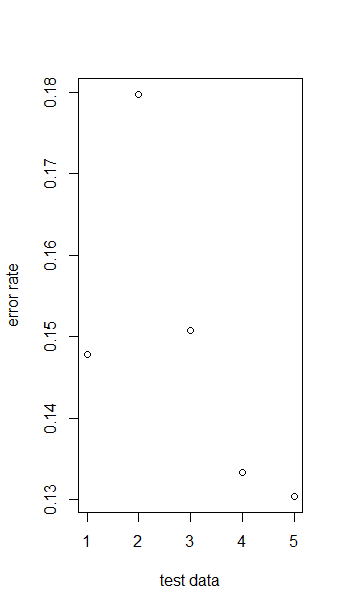
\includegraphics[width=100mm, scale = 0.5]{carError.png}
  \caption{car data error rate}
\end{figure}
\begin{figure}
  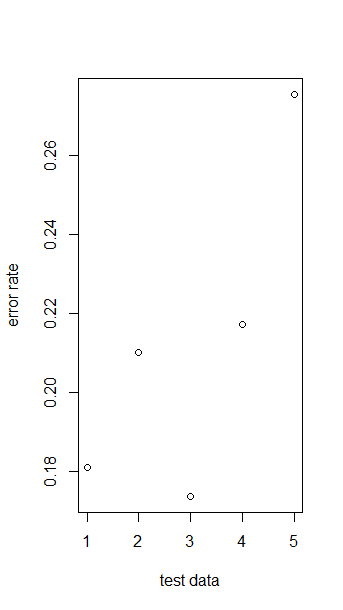
\includegraphics[width=100mm, scale = 0.5]{creditError.png}
  \caption{car data error rate}
\end{figure}
\item[\textbf{3.2}] Pick the optimal Naive Bayes classifiers (one for  car evaluation  data set and  another one for credit approval data set.) from question 3.1 and compare them with your best KNN models from question 2. Discuss the performances of the optimal classifiers over car evaluation and credit approval data sets, i.e, which one performed better? 
\paragraph{}
The optimal Naive Bayes classifier's  error rate  for car data is 0.13. However, the best KNN model's error rate is 0.026. \\
On the credit data set, the optimal Naive Bayes classifier's error rate is 0.17, and the best KNN model's error rate is 0.25.\\
As a result, Naive Bayer perfroms better on the credit data set, KNN works better on the car data set on the other hand.
\end{enumerate}
\section*{Problem 4 [10 points]} 

From textbook, Chapter 5 exercise 7 (Page 318)
\paragraph{7a}
$P(A = 1| -)=\frac{2}{5}\\$
$P(A = 0| -)= \frac{3}{5}\\$
$P(A = 1| +) = \frac{3}{5}\\$
$P(A = 0| +) = \frac{2}{5}\\$
$P(B = 1| -)=\frac{2}{5}\\$
$P(B = 0| -)=\frac{3}{5}\\$
$P(B = 1| +) = \frac{1}{5}\\$
$P(B = 0| +) = \frac{4}{5}\\$
$P(C = 1| -) = 1\\$
$P(C = 0| -) = 0\\$
$P(C = 1| +) = \frac{4}{5}\\$
$P(C = 0| +) = \frac{1}{5}\\$
\paragraph{7b}
$P(+|A=0, B=1,C=0) = P(A = 0|+)P(B = 1|+)P(C = 0|+) * P(+) = 0.4 * 0.2 * 0.2 * 0.5 = 0.008$\\
$P(-|A=0, B=1,C=0) = P(A = 0| -)P(B = 1| -)P(C = 0| -) * P(-) = 0$\\
$0.008 > 0$\\
Therefore, The test sample belongs to class '+'
\paragraph{7c}
$P(A = 0| -) = \frac{3 + 2}{5 + 4} = \frac{5}{9}\\$
$P(A = 0| +) = \frac{2 + 2}{5 + 4} = \frac{4}{9}\\$
$P(B = 1| -) = \frac{2 + 2}{5 + 4} = \frac{4}{9}\\$
$P(B = 1| +) = \frac{1 + 2}{5 + 4} = \frac{1}{3}\\$
$P(C = 0| -) = \frac{0 + 2}{5 + 4} = \frac{2}{9}\\$
$P(C = 0| +) = \frac{1 + 2}{5 + 4} = \frac{3}{9}\\$
\paragraph{7d}
$P(+|A=0, B=1,C=0) = P(A = 0|+)P(B = 1|+)P(C = 0|+) * P(+) = \frac{4}{9} * \frac{1}{3} * \frac{3}{9} * \frac{1}{2} = \frac{12}{486} = 0.024$\\
$P(-|A=0, B=1,C=0) = P(A = 0| -)P(B = 1| -)P(C = 0| -) * P(-) =  \frac{5}{9} * \frac{4}{9} * \frac{2}{9} * \frac{1}{2} = \frac{40}{1458} = 0.027$\\
$0.027 > 0.024$\\
Since the probability of classified '-' is larger, the label should be '-'
\paragraph{7e}
Since the probability of C = 0 given C is '-' is 0, which makes the test sample equal to 0. However, we do not want the probability to be zero when we trying to predict to test case. Therefore, the m-estimate is better in this approach.
 %%%%%%%%%%%%%%%%%%%%%%%%%%%%%%%%%%%%%%
%                   EXTRA CREDIT
 %%%%%%%%%%%%%%%%%%%%%%%%%%%%%%%%%%%%%%
  \section*{Extra Credit [30 points]} 
\begin{itemize}
\item From textbook, Chapter 5 exercises 8, 17 (Pages 318 $\&$ 322) \textbf{[15 points}]
\paragraph{8a}
$P(A = 1|-)=\frac{2}{5}\\$
$P(A = 1|+) = \frac{3}{5}\\$
$P(B = 1|-)=\frac{2}{5}\\$
$P(B = 1|+) = \frac{2}{5}\\$
$P(C = 1|-)=\frac{1}{5}\\$
$P(C = 1|+) = \frac{4}{5}\\$
\paragraph{8b}
$P(+|A = 1, B = 1, C = 1) = P(A = 1|+) × P(B = 1|+) × P(C = 1|+) = \frac{3}{5} * \frac{2}{5} * \frac{4}{5} = \frac{24}{125}$\\
$P(-|A = 1,B = 1, C = 1) = P(A = 1|-) × P(B = 1|-) × P(C = 1|-)= \frac{2}{5} * \frac{3}{5} * \frac{1}{5} = \frac{6}{125}$\\
$\frac{24}{125} > \frac{6}{125}$\\
The test sample is assigned to '+'\\
\paragraph{8c}
$P(A = 1) * P(B = 1) = \frac{5}{10}* \frac{4}{10} = \frac{1}{5}$\\
$P(A = 1, B = 1) = \frac{2}{10} = \frac{1}{5}$\\
$P(A = 1) * P(B = 1) = P(A = 1, B = 1)$\\
They are independent
\paragraph{8d}
$P(A = 1) * P(B = 0) = \frac{5}{10}* \frac{6}{10} = \frac{3}{10}$\\
$P(A = 1, B = 0) = \frac{3}{10}$\\
$P(A = 1) * P(B = 0) = P(A = 1, B = 0)$\\
They are independent
\paragraph{8e}
$P(A = 1| +) * P(B = 1|+) = \frac{6}{10}* \frac{4}{10} = \frac{24}{100}$\\
$P(A = 1, B = 1| +) = \frac{2}{10}$\\
$P(A = 1|+) * P(B = 1|+) \neq P(A = 1, B = 1|+)$\\
They are not independent
\item Problem 1: $K$-fold cross validation implementation  \textbf{[15 points}]
\end{itemize}




%%%%%%%%%%%%%%%%%%%%%%%%%%%%%%%%%%%%%%
\section*{What to Turn-in}
 Submit a .zip file that includes the files below. Name the .zip  file as \quotes{usename-section number}, i.e., hakurban-B365.


\begin{itemize}
\item The *tex and *pdf of the written answers to this document.
\item *\texttt{R}files for:
\begin{itemize}
\item Question 1: \textsf{crossValidation.R}, output of cross validation: training  and test data sets 
\item Question 2.1: \textsf{knn.R}, Question 2.3: \textsf{knnValidation.R}
\item Question 3: \textsf{naiveBayes.R}
\end{itemize} 
\item A README file that explains how to run your code and other files in the folder
\end{itemize}




\end{document}


